%
% cauchy.tex -- tikz image container for Cauchy problem
%
% (c) 2019 Prof Dr Andreas Müller, Hochschule Rapperswil
%
\documentclass[tikz,12pt]{standalone}
\usepackage{amsmath}
\usepackage{times}
\usepackage{txfonts}
\usepackage{pgfplots}
\usepackage{csvsimple}
\usetikzlibrary{arrows,intersections,math}
\begin{document}
\begin{tikzpicture}[>=latex]

\node at (0,0) {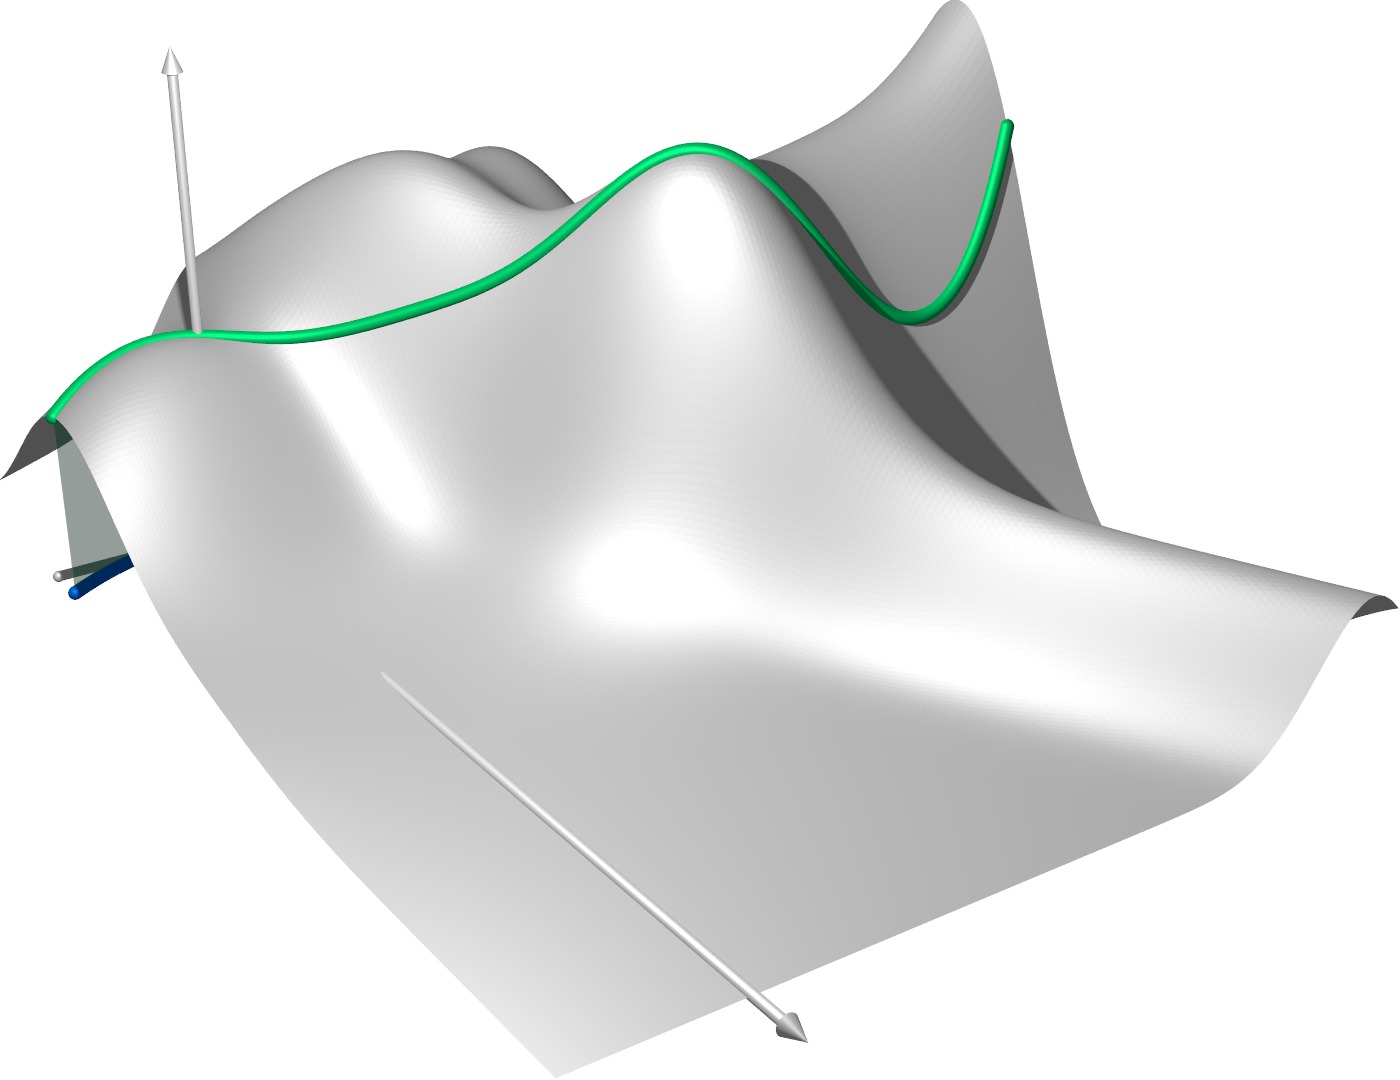
\includegraphics[width=15cm]{cauchy.jpg}};

\node at (1.3,-5.2) {$x$};
\node at (-5.5,5.4) {$z$};

\end{tikzpicture}
\end{document}

